\section{Fundamental of Causal Inference}
\subsection{Motivation}
\begin{frame}{What is Causality?}
\begin{block}{A definition from Wikipedia}
\textbf{Causality} (also referred to as causation) is the relationship
between an event (\textit{the cause}) and a second event (\textit{the effect}),
where the second event is understood as a consequence of the
first.
\end{block}\pause
\textbf{An example in real life} : Does smoking cause lung cancer?\\
\pause	
\begin{center}
\alert{Yes, it might be!}
\end{center}
\end{frame}
\begin{frame}{From Probabilistic View }
\textbf{Problem:} Does smoking cause lung cancer?\pause
\begin{center}
\begin{itemize}
\item Smoking does \alert{increase the probability} of getting lung cancer.
\end{itemize}
\end{center}
\end{frame}
\begin{frame}{Statistical Inference Overview}
\begin{figure}
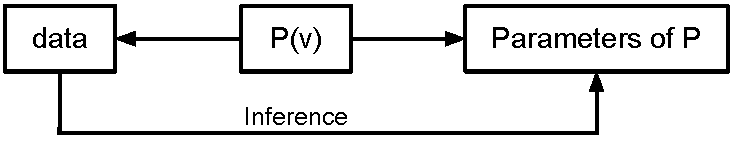
\includegraphics[scale=0.7]{imgs/statInf}
\end{figure}
\begin{itemize}
\item Approximate an estimate of $X$ given evidence $e$, namely, $Pr(X\,|\,e)$. E.g., Regression or Classification problems.
\item Rejection of hypothesis, i.e., assert wether samples are from a certain distribution.  
\item Confidence interval, i.e., construct an interval based on dataset 
\end{itemize}
\end{frame}
\begin{frame}{Causal Inference Overview}
\begin{figure}
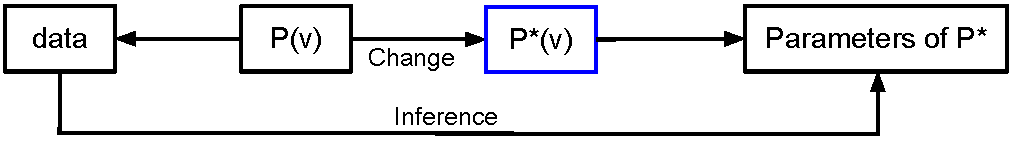
\includegraphics[scale=0.6]{imgs/causalInf}
\end{figure}
\begin{itemize}
\item What if $P$ has shifted itself to $P^*$?
\item<2-> \textbf{Key factors:} Causes, Changes, and Invariants . 
\item<2-> Inference of $P^*$ and reasoning of changes. 
\end{itemize}
\end{frame}
\begin{frame}{What makes Causal Inference interesting?}
\begin{itemize}
\item Human understands the world in terms of causes and effects.
\item Empirical science is about establishing causes.
\item Causal inference gives a mathematical language for causal
statements, and tools to solve causal problems formally.
\item Alternative exercising to decision making, reasoning, etc.
\end{itemize}
%\begin{alertblock}{Note}
%Causal Inference has fundamental difference with machine learning
%\end{alertblock}
\end{frame}
\subsection{Causal Graphical Model}
\begin{frame}{Association}
\begin{itemize}
\item Now we want to find out what \alert{causes} lung cancer
\end{itemize} \pause
\begin{columns}
\begin{column}{0.5\textwidth}
\begin{table}
\centering
\begin{tabular}{|c|c|c|c|}
\hline
& & \multicolumn{2}{|c|}{Lung cancer}\\\hline
smoking & yellow teeth & yes & no\\\hline
yes & yes & 100 & 400\\\hline
yes & no & 100 & 400\\\hline
no & yes & 1 & 450\\\hline
no & no & 9 & 8540\\\hline
\end{tabular}
\caption{Data observations from 10000 people}
\end{table}
\end{column}\hfill
\begin{column}{0.5\textwidth}
\vspace*{-0.5in}
\begin{figure}
\centering
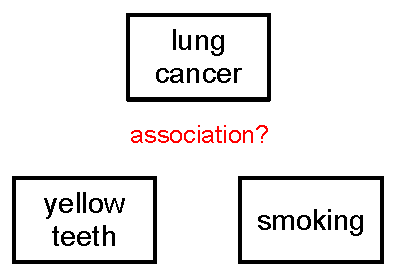
\includegraphics[scale=0.6]{imgs/smokepl}
\end{figure}
\end{column}
\end{columns}
\end{frame}
\begin{frame}{Measurements of Association}
\textbf{To find out associations among variables}
\begin{itemize}
\item Mutual information (Information theory)
\item Pearson (linear) correlation
\item Spearman's rho (rank correlation)
\item Effect size between two variables
\item Many others
\end{itemize}
\end{frame}
\begin{frame}{Observations from Data}
\textbf{Obviously}
\begin{itemize}
\item \textit{yellow teeth} and \textit{lung cancer} are associated.
\end{itemize}\pause
\alert{\textbf{But...}}
\begin{itemize}
\item Bleaching the teeth does not help reduce the probability
of getting lung cancer.
\end{itemize}\pause
\begin{alertblock}{Caution!}
Correlation does not imply Causation
\end{alertblock}
\end{frame}
\begin{frame}{Statistical Implication}
\begin{block}{Reichenbach's \textit{Common Cause Principle}}
If $X$ and $Y$ are correlated, then either $X$ causes $Y$ or $Y$ causes $X$ or they share a latent common cause $Z$.
\end{block}
\begin{figure}
\setcounter{subfigure}{0}
	\centering
	\begin{subfigure}[H]{0.3\textwidth}
		\centering
		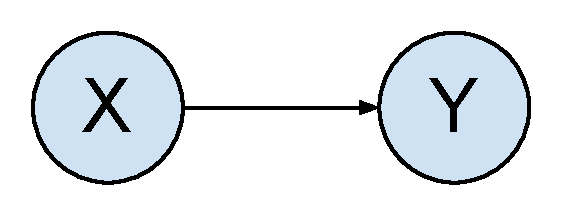
\includegraphics[scale=0.3]{imgs/x2y}
		\caption{$X$ causes $Y$}
		%\label{}	
	\end{subfigure}
	\begin{subfigure}[H]{0.3\textwidth}
		\centering
		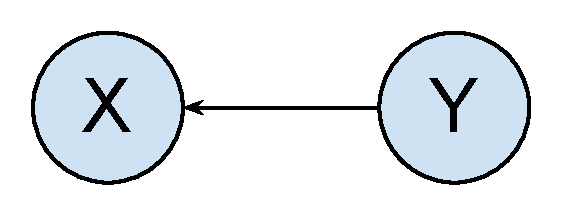
\includegraphics[scale=0.3]{imgs/y2x}
		\caption{$Y$ causes $X$}
		%\label{}	
	\end{subfigure}
	\begin{subfigure}[H]{0.3\textwidth}
		\centering
		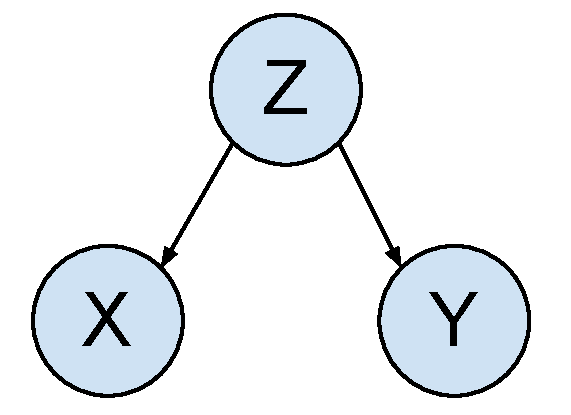
\includegraphics[scale=0.3]{imgs/z2xy}
		\caption{A common latent cause $Z$}
		%\label{}	
	\end{subfigure}
\end{figure}\pause
\begin{itemize}
\item<+-|alert@+> It links causality with probability
\end{itemize}
\end{frame}
\begin{frame}{Functional Causal Model (pearl et al.)} 
\begin{itemize}[<+->]
\item A set of variables (factors) $\left\lbrace X_1,\ldots,X_n \right\rbrace$
\item Directed acyclic graph $\mathcal{G}$ with vertices $\left\lbrace X_1,\ldots,X_n \right\rbrace$
\item Parents of node $X_i$ in $\mathcal{G}$ are its direct causes
\item $X_i=f_i(Parents(X_i),\epsilon_i)$, where $\left\lbrace\epsilon_1,\ldots,\epsilon_n\right\rbrace$ are jointly independent noises
\item The above entails a joint probability distribution $P(X_1,\ldots,X_n)$
\item Problems are twofold:
      \begin{enumerate}
		\item How is the $P$ like?
		\item Can we recover $\mathcal{G} from P$? 
	\end{enumerate}
\item[] \begin{textblock*}{200mm}(0.6\textwidth,-2cm)
		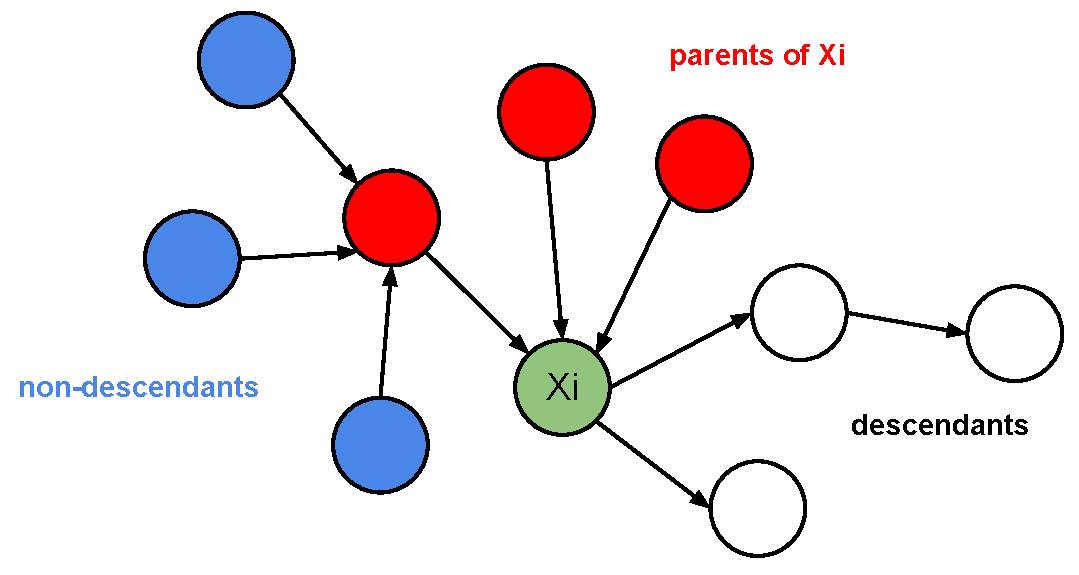
\includegraphics[scale=0.25]{imgs/causalgm}
	\end{textblock*}
\end{itemize}
\end{frame}
\begin{frame}{Functional Causal Model, ctd.}
The following are equivalent:
\begin{itemize}
\item A functional causal model exists
\item Local causal Markov condition: $X_i$ is statistically independent of its non-descendants given $X_i$'s parents
\item Global Causal Markov condition: \textbf{d-separation} characterize the set of independences over all the observables
\item Factorization: $P(X_1,\ldots,X_n)=\prod_iP(X_i\,|\,Parents(X_i))$
\end{itemize}
\end{frame}
\begin{frame}{Learning causation from Data?}
\begin{block}{Question}
Given observational data, can we infer $\mathcal{G}$?
\end{block}
\begin{itemize}
\item \textbf{Simple answer:} impossible without additional information
\item Possible with interventions (outside force, empirical treatment, etc.)
\item By conditional independence tests, \textit{Markov equivalence class} containing $\mathcal{G}$ can be learned. \alert{But}, it fails in simplest 2-nodes case.
\item 2-nodes case can be tackled applying residual dependence test. (see Hoyer et al.)
\end{itemize}
\end{frame}
\begin{frame}{Markov Equivalence Class}
\textbf{Simplest case with three variables}
\begin{itemize}
\item[]<1-> \begin{figure}
\setcounter{subfigure}{0}
			\begin{subfigure}[H]{0.4\textwidth}
			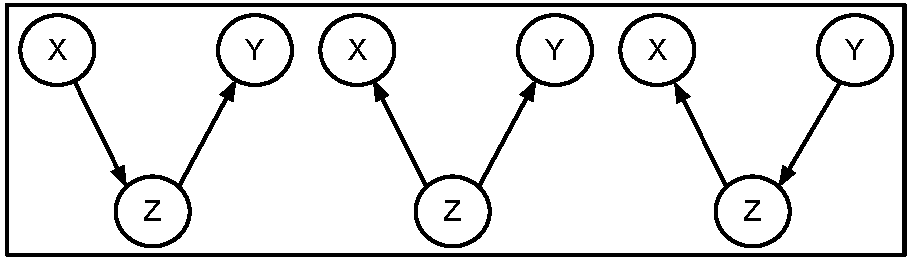
\includegraphics[scale=0.4]{imgs/eqv}
			\caption{Equivalence}
			\end{subfigure}\hfill
			\begin{subfigure}[H]{0.3\textwidth}
			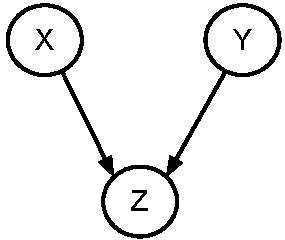
\includegraphics[scale=0.4]{imgs/noneqv}
			\caption{Non-equivalence}
			\end{subfigure}
		\end{figure}
\item<2-> Samples can be explained by all graphs in equivalence class
\item<3-> For example:
\begin{table}
\centering
\begin{tabular}{|c|c|}
\hline
Equivalence class & Non-equivalence class \\\hline
$Dep(X,Z\,|\,\emptyset)$ & $Dep(X,Z\,|\,\emptyset)$\\\hline
$Dep(Y,Z\,|\,\emptyset)$ & $Dep(Y,Z\,|\,\emptyset)$\\\hline
$Dep(X,Y\,|\,\emptyset)$ & \alert{$Ind(X,Y\,|\,\emptyset)$}\\\hline
$Ind(X,Y\,|\,Z)$ & \alert{$Dep(X,Y\,|\,Z)$}\\\hline
\end{tabular}
\end{table}	
\end{itemize}
\end{frame}